\subsection{複数要素のシミュレーション}

\begin{figure}[b]
\begin{center}
\psfrag{0}{0}
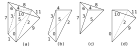
\includegraphics[width=\hsize]{triprism_decomp.eps}
\caption{三角柱を3つの四面体に分解}
\end{center}
\end{figure}

本節では1要素のシミュレーションを複数要素に拡張します。解くべき方程式は
\begin{align}
\left\{
\sum_k
\left[
{\mu_i}^{-1} R_k
-\omega\left(\omega\epsilon_k+j\sigma_k\right)S_k
\right]
\right\}
\textbf{v}
=\sum_k \textbf{e}_{1,k}+\sum_k\textbf{e}_{2,k}+\sum_k\textbf{e}_{3,k}
\end{align}
です。右辺は1要素シミュレーションと同様の電流励起です。左辺においては
\begin{align}
R_{k,g(l),g(m)} &= r_{k,l,m}\\
S_{k,g(l),g(m)} &= s_{k,l,m}
\end{align}
です。$R_k, r_k, S_k, s_k$ とその添字(そえじ)の関係を図?に示します。
$R_k, S_k$ はエッジ数の大きさを持つ正方行列です。
$r_k, s_k$ は大きさ 4 の正方行列で,
前節の1メッシュシミュレーションでの$r, s$に相当します。
1番目の添え字(ここでは$k$)はメッシュ番号を表します。
2番目の添え字(ここでは$g(l), l$)は行列
$R_k, r_k, S_k, s_k$ の行番号を表します。
3番目の添え字(ここでは$g(m), m$)は行列
$R_k, r_k, S_k, s_k$ の列番号を表します。
$g$はローカルエッジ番号をグローバルエッジ番号に変換する関数です。
各メッシュ毎に $r_k, s_k$ を計算しそれに係数を掛けグローバルな
$R_k, S_k$ に加算すればよいことになります。
これを行うコードをリスト?に示します。
この関数を使用して図?に示す例題を1つずつシミュレーションしていきます。
